\documentclass[11pt]{article}
\usepackage{graphicx}  % Include figure files
\usepackage{amsmath}

\begin{document}

\section*{Reply from Tuesday, Aug. 11, 2020}

We will show that the specific value of efficiency does not impact the quality of the experimental result.
However, the stability of the efficiency ratio is essential, see below.

Let us evaluate in detail the influence of the hadron efficiencies, $\eta_n$ and $\eta_p$, on the experimental result.
%and proton efficiency $R_{\eta_{n/p}} = \eta_n/\eta_p$ on the measurement of $R_{corrected} = R_{n/p} \times f_{corr}$ and $S^n$.
The $S^n$ result is sensitive only to the ratio of neutron efficiency to proton efficiency, $R_{\eta} = \eta_n/\eta_p$.
Such a ratio is very stable because the nucleon momenta are the same by definition of the Rosenbluth method.   
We have a plan to monitor the stability of this ratio in our experimental data.

Our primary experimental observable is the ratio of yields $R_{n/p} = N_{en}/N_{ep}$.
In this experiment, the parameter of interest is $A = [R_{n/p, \epsilon-1}/R_{n/p, \epsilon-2}]\times[R_{\eta, epsilon-1}/R_{\eta, epsilon-2}]$.

As we wrote in our proposal, pages 12 and 13, and under the assumption that the reduced cross section $\sigma_R$ is linear in $\epsilon$,
the neutron Rosenbluth slope $S^n$ can be obtained as:
%
\begin{equation}
  S^n = \frac{A-1}{\Delta\epsilon} + S^p = (\frac{R_{n/p, \epsilon-1}}{R_{n/p, \epsilon-2}}\times \frac{R_{\eta, epsilon-1}}{R_{\eta, epsilon-2}}-1)/\Delta\epsilon + S^p
  \label{eq:Sn}
\end{equation}
%
As it is easy to see from the formula above, the efficiency impact cancels out in $S^n$ if the efficiency ratio is stable.

The procedure to evaluate the hadron detector efficiency was presented on the Monday write-up (see below).
The result will be fitted by a few parameter functions, and the ratio of efficiency $R_{\eta}$ is characterized by those parameters as well as the threshold.
This study will be performed for all modules of HCal used in the experiment.
After the data collection, we will repeat this study with the recorded data for each kinematic.
Based on projected statistics of a few million events, the accuracy of $R_{\eta}$ will be better than 0.1\%.
With such an accuracy, we will monitor the stability of $R_{\eta}$.
This corresponds to the uncertainty in $S^n$, using the formula above, of 0.004, with our $\Delta \epsilon = 0.24$. 

Additional analysis of the efficiency ratio is presented on Fig~\ref{fig:Reta_np}.
This analysis focused on absolute value of efficiency ratio, for which we expect 1\% statistical level.
To monitor the stability, we will have hundreds of times more statistics.
%
\begin{figure}[!h]
  \centering
  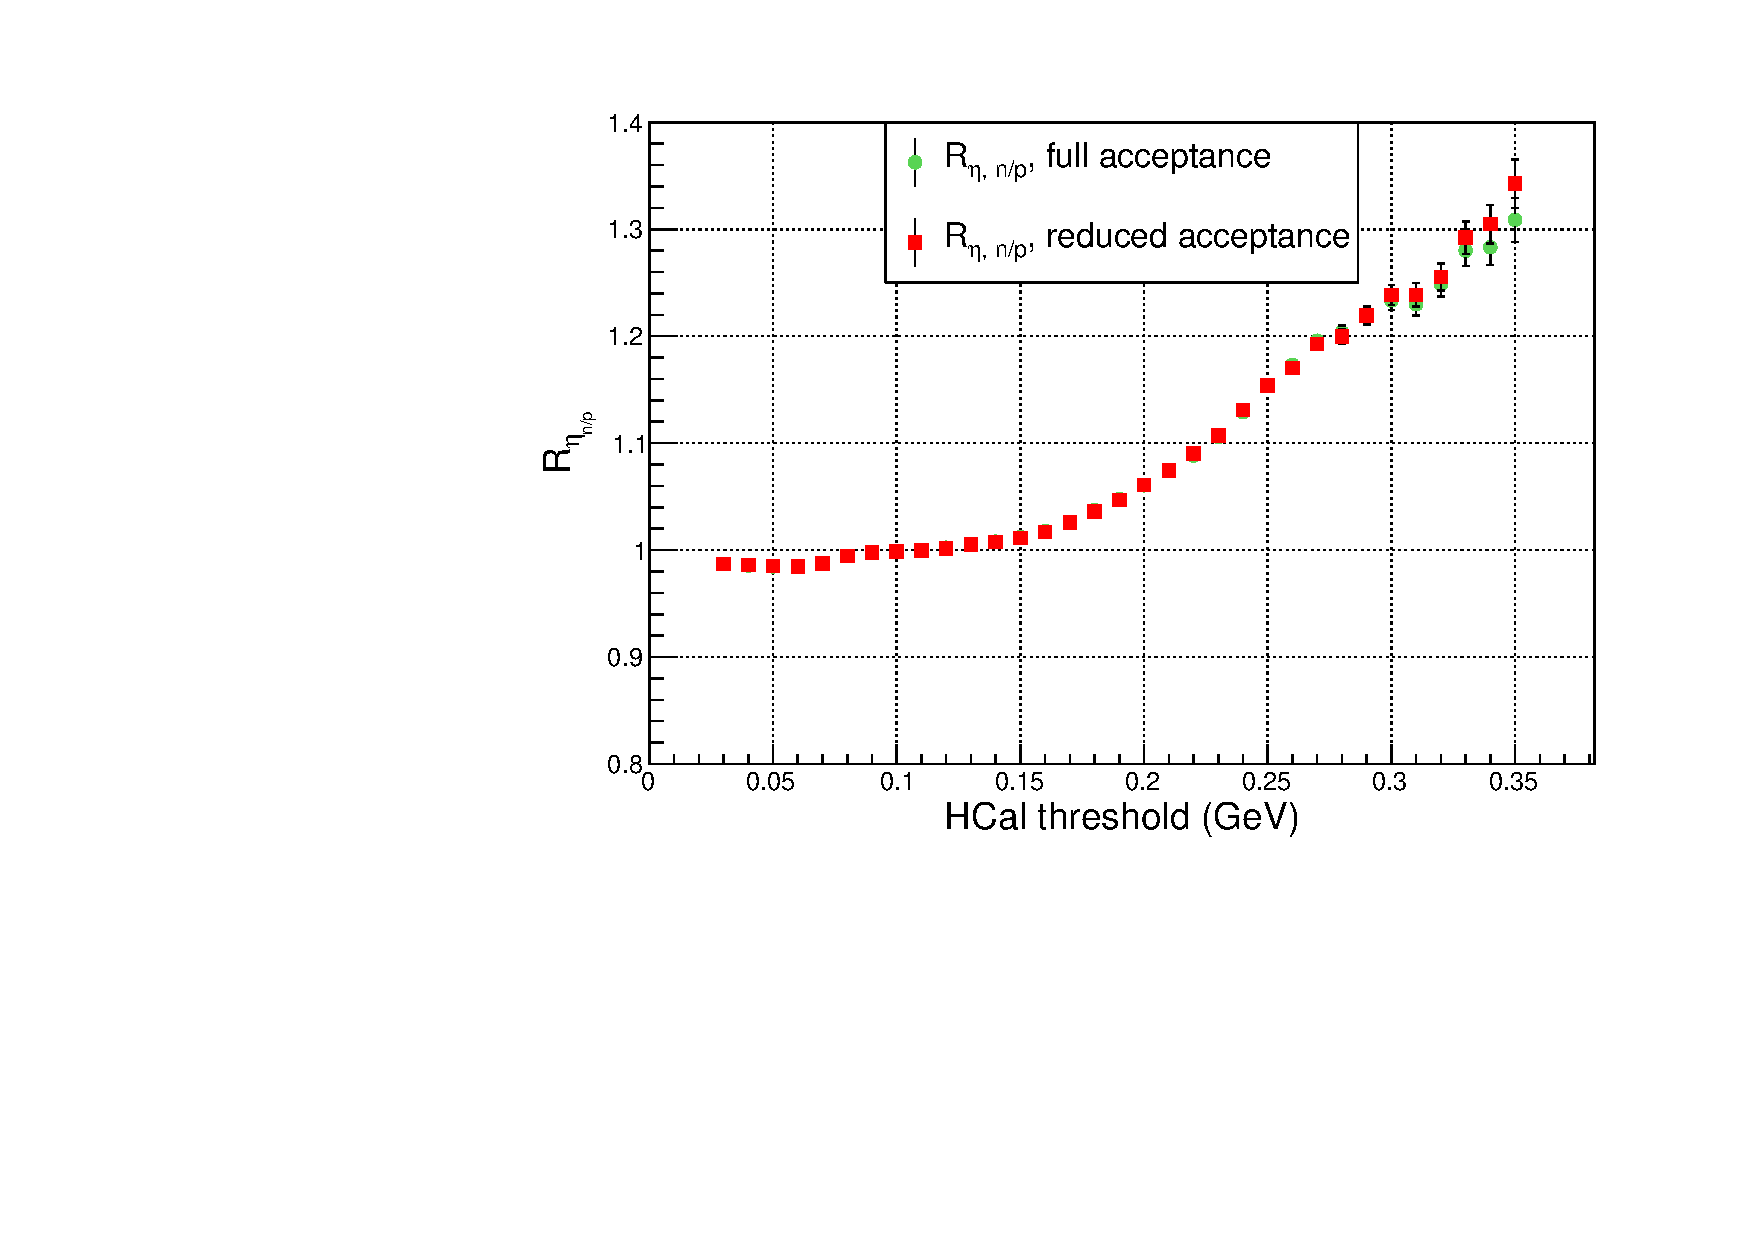
\includegraphics[width=7cm]{Reta_np_fthr_errs.pdf}
  \caption{Neutron/proton efficiency ratio $R_{\eta_{n/p}}$ as a function of the calorimeter threshold, for our quasi-elastic sample. The error bars represent the uncertainty from the calibration measurements discussed earlier. The green represents $R_{\eta_{n/p}}$ on the full acceptance, the red represents $R_{\eta_{n/p}}$ on a reduced acceptance. %The discrepancy between the two (blue) is about 0.1\% below a threshold of 0.15 GeV.%, but becomes about 0.5\% between 0.15 and 0.3 GeV, up to 1\% beyond 0.3 GeV}
            }
  \label{fig:Reta_np}
\end{figure}
%
\newpage

\section*{Reply from Monday, Aug. 10, 2020}

Simulated efficiencies were obtained from the amplitude distributions like the ones shown as in the histograms in Fig.~\ref{fig:Neff}.
For example, with threshold 100 MeV the efficiency for the proton is 90.8\% (Fig.~\ref{fig:Neff}~{\bf(a)}) Similar distribution for the neutron in Fig.~\ref{fig:Neff}~{\bf(b)} leads to 92.0\% efficiency for the same threshold.\\
The efficiency $\eta_{n}$ is calculated as the ratio of the number of events with energy deposit above 0.10 GeV over the total number of events.
%
\begin{figure}[!h]
  \centering
  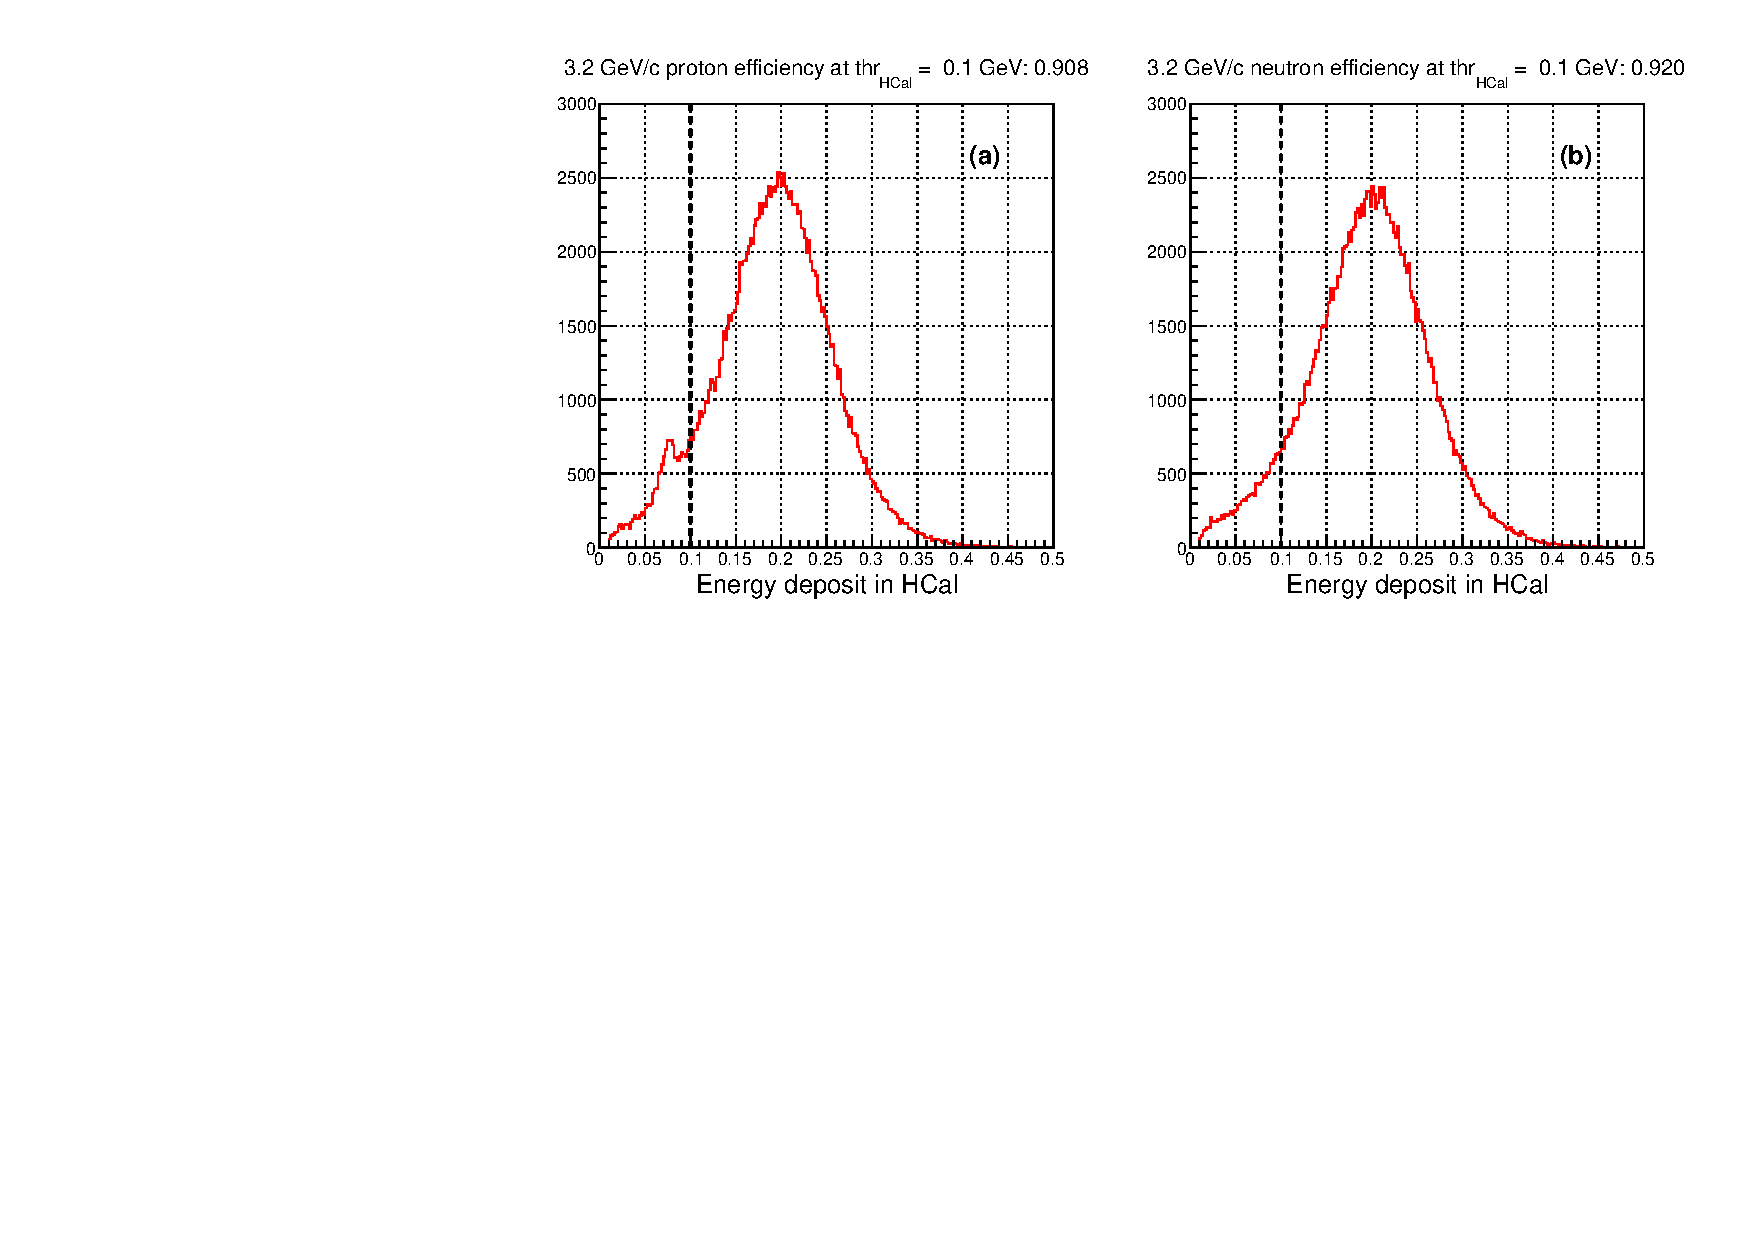
\includegraphics[width=12cm]{ProtVsNeut_MC.pdf}
  \caption{Amplitude signal expected in HCal for the protons~{\bf(a)} and the neutrons~{\bf(b)}. The efficiency is shown for a 0.1 GeV threshold.}
  \label{fig:Neff}
\end{figure}
%
%To dissipate any misunderstanding: the 90\% ``efficiency'' with 0.1 GeV quoted elsewhere (proposal, presentation) represents the fraction of quasi elastic 3.2 GeV/c nucleons which, if they deposit any energy in HCal, deposit 0.1 GeV or more. The efficiencies quoted in this document includes the small fraction of cases (about 5\%) when the nucleon does not give any signal at all.
%
%\begin{figure}[!h]
%  \centering
%  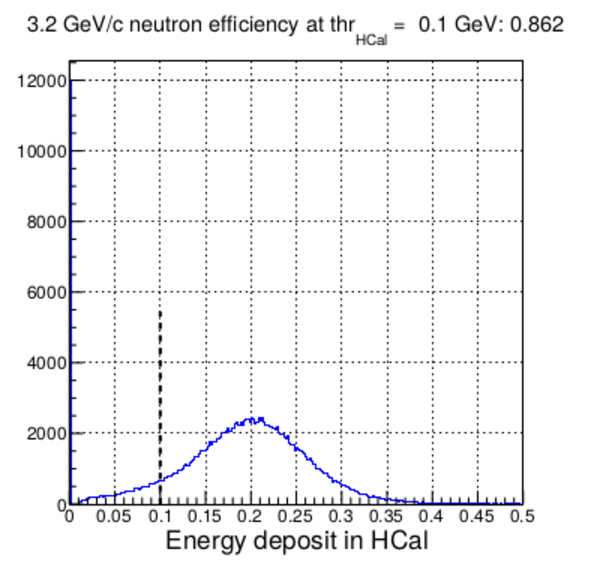
\includegraphics[width=5cm]{Neut_Eff_MC.pdf}
%  \caption{Neutron amplitude signal expected in HCal.}
%  \label{fig:neff}
%\end{figure}
%

We also would like to show how the efficiency will be measured.
This will be done by using "elastic" reactions H$(e,e’)p$, H$(\gamma,\pi^+)n$
and more with D$(\gamma,\pi^+)n$ and D$(\gamma,\pi^-)p$ single pion production.
Fig.~\ref{fig:Nproj}~{\bf(a)} shows the projected proton position from H$(e,e’)p$, 
Fig.~\ref{fig:Nproj}~{\bf(b)} shows the projected proton position from H$(\gamma,\pi^+)n$.
%
\begin{figure}[!h]
  \centering
  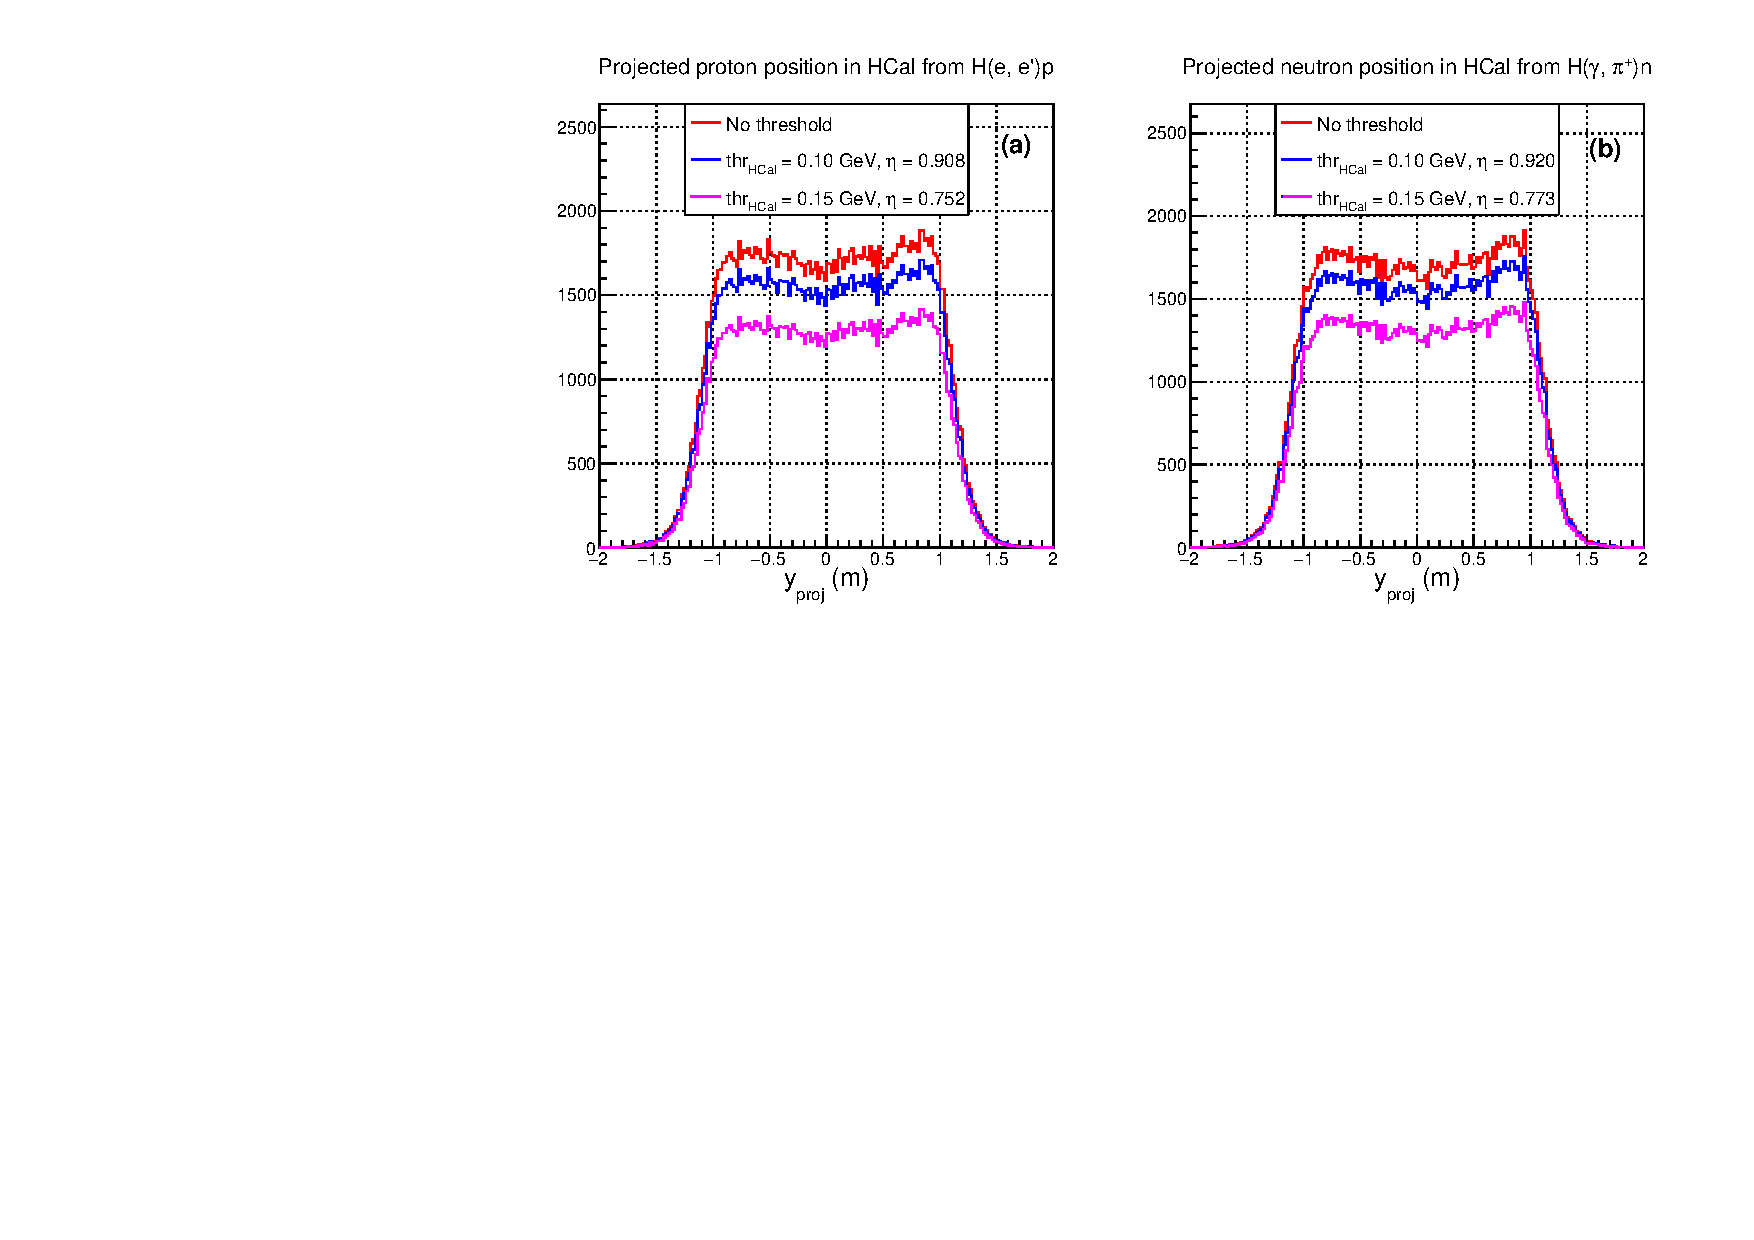
\includegraphics[width=12cm]{ProtVsNeut_CalibYproj.pdf}
  \caption{Projected position in HCal in for the protons in H$(e,e’)p$~{\bf(a)} and the neutrons in H$(\gamma,\pi^+)n$~{\bf(b)}. On both panels, red distributions show the projected distribution for $p$, $n$, not detected; blue distributions show the distribution for $p$, $n$ detected with a 0.1 GeV threshold; magenta distributions show the distribution for $p$, $n$ detected with a 0.15 GeV threshold.}
  \label{fig:Nproj}
\end{figure}
%
In each case, the trigger will not use the nucleon detector information.
Analysis will use the amplitude distribution in the same way as done on  Fig.~\ref{fig:Neff} with the red distributions.
Blue distributions on Fig.~\ref{fig:Nproj} show the expected Y distribution applying a 0.10 GeV threshold on HCal;
Magenta distributions on Fig.~\ref{fig:Nproj} show the expected Y distribution applying a 0.15 GeV threshold on HCal.
As reported in the E12-09-019 GMn proposal\footnote{https://www.jlab.org/exp\_prog/proposals/09/PR12-09-019.pdf} on Table~8, the expected recorded statistics for H$(\gamma,\pi^+)n$ are of the order of 4000 events, which will represent a relative 1.5\% uncertainty on the neutron efficiency. The recorded statistics for H$(e,e’)p$ are of the order of 82000 events, which will represent a relative 0.3\% uncertainty on the proton efficiency.\\

\iffalse
We also want to underline that the uncertainty on the nucleon efficiency $\eta_N$ will not be a major contributor to the uncertainty on the neutron Rosenbluth slope $S^n$. The relative uncertainty on $S^n$ due to $\eta_N$ is:
%
\begin{equation}
  \Delta S^n/S^n \simeq \Delta\eta_N/\eta_N 
\end{equation}
%
which gives, assuming $\eta_N$ close to 0.9
%
\begin{equation}
  \Delta S^n \simeq S^n \Delta\eta_N = 0.14\%
\end{equation}
%
\fi

\end{document}
